\section{Technologie}
\begin{frame}{\insertsection}
	\begin{block}{Architektura klient-serwer}
		Pozwala określić komunikację między klientem, a serwerem.
	\end{block}
	\begin{figure}
		\centering
		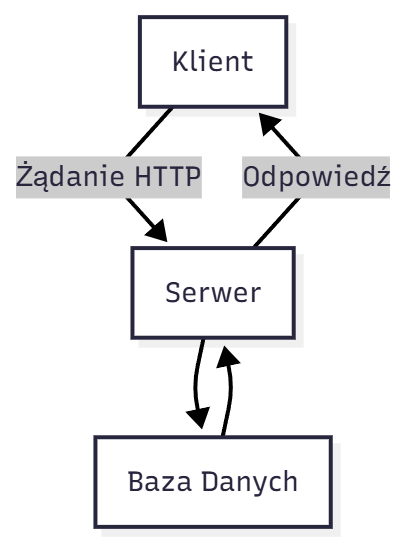
\includegraphics[height=6cm,width=0.5\linewidth]{../images/Klient-Serwer}
		\label{fig:klient-serwer}
	\end{figure}
\end{frame}

\begin{frame}{\insertsection}
	\begin{block}{Java}
		 Język zapewniający ogromne możliwości.
	\end{block}
\begin{figure}
	\centering
	
\includegraphics[width=0.9\linewidth]{../images/javaLogo}
	\label{fig:javalogo}
\end{figure}
\end{frame}

\begin{frame}{\insertsection}
	\begin{block}{Spring Boot}
		Upraszcza tworzenie, konfigurację i uruchamianie aplikacji.
	\end{block}
	\begin{figure}
		\centering
		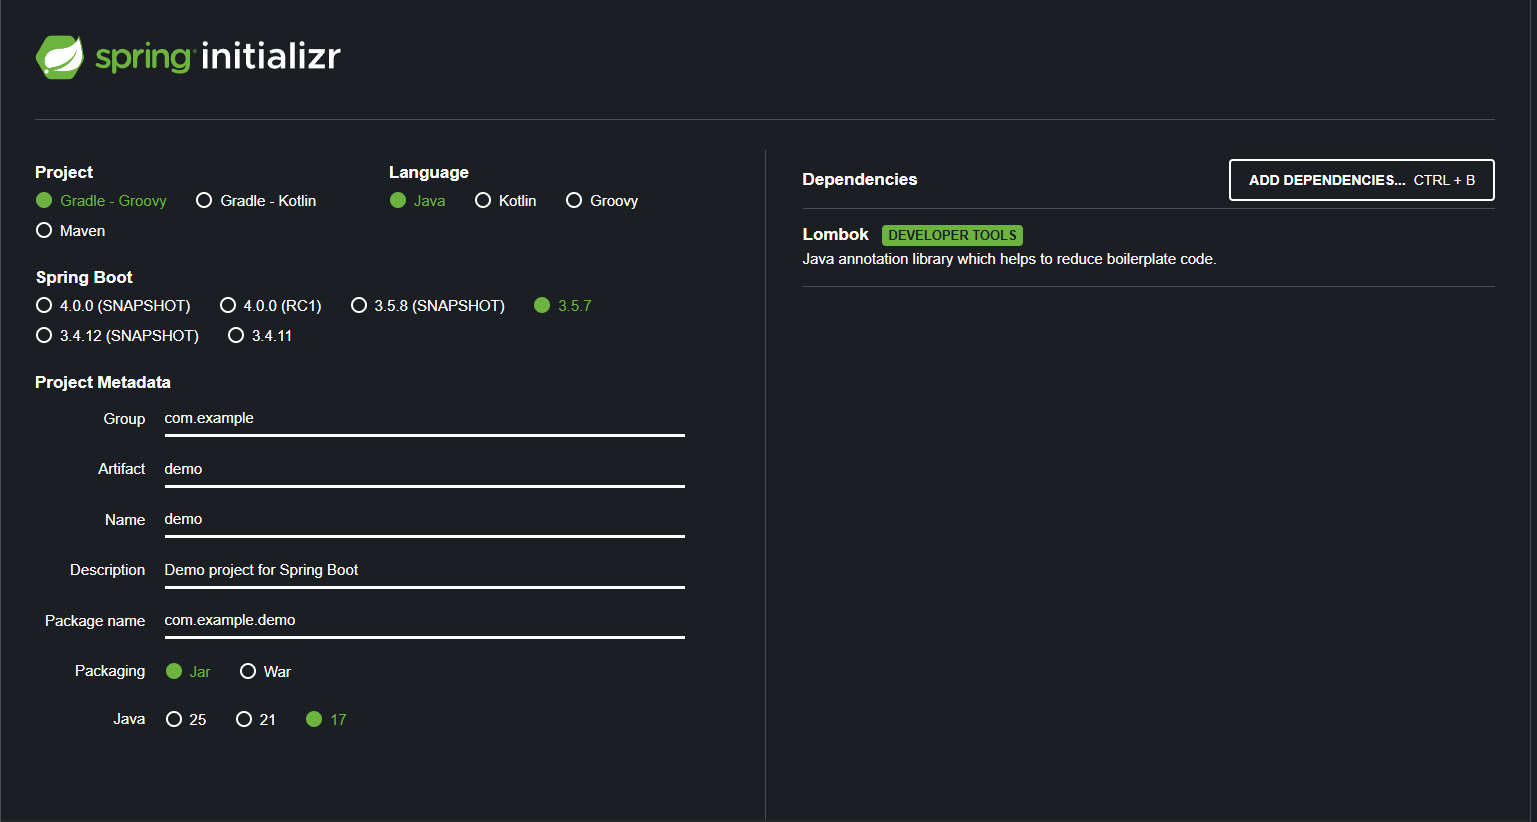
\includegraphics[width=0.9\linewidth]{../images/springInit}
		\label{fig:springinit}
	\end{figure}
\end{frame}

\begin{frame}{\insertsection}
	\begin{block}{Maven}
		Zarządzanie projektem.
	\end{block}
	\begin{figure}
		\centering
		
\includegraphics[width=0.9\linewidth]{../images/MavenLogo}
		\label{fig:mavenlogo}
	\end{figure}
\end{frame}

\begin{frame}{\insertsection}
	\begin{columns}
		\column{0.45\textwidth}
		\begin{minipage}[t][6cm][t]{\linewidth}
			\begin{block}{React}
				Biblioteka do tworzenia aplikacji webowych.
			\end{block}
			\vfill
			\centering
			
\includegraphics[height=2.2cm,keepaspectratio]{../images/ReactIcon}
		\end{minipage}
		\column{0.45\textwidth}
	 	\begin{minipage}[t][6cm][t]{\linewidth}
			\begin{block}{Język TypeScript}
				Język umożliwiający statyczne typowanie.
			\end{block}
			\vfill
			\centering
			
\includegraphics[height=2.2cm,keepaspectratio]{../images/TypeScript}
		\end{minipage}
	\end{columns}
\end{frame}

\begin{frame}{\insertsection}
	\begin{block}{MongoDB}
		Nierelacyjna baza danych, przechowująca dane w postaci dokumentów
	\end{block}
	\begin{columns}
		\column{0.2\textwidth}
			\begin{figure}
			\centering
			
\includegraphics[width=1\linewidth]{../images/MongoLogo}
			\label{fig:mongologo}
		\end{figure}
		\column{0.75\textwidth}
			\begin{figure}
			\centering
			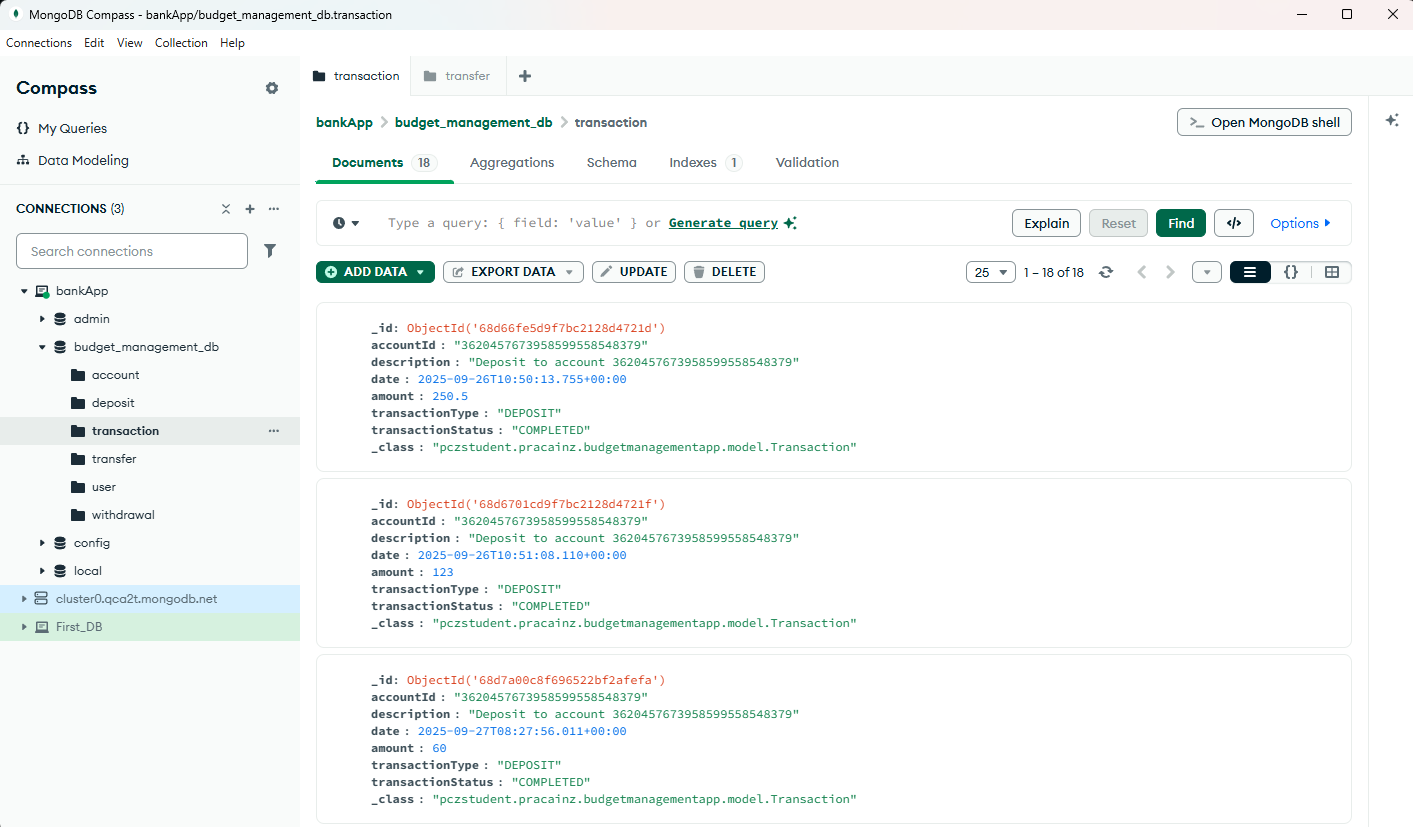
\includegraphics[width=1\linewidth]{../images/MongoData}

			\label{fig:mongodata}
		\end{figure}
	\end{columns}
\end{frame}
